%\documentclass[a4paper,twoside,11pt,open=any]{scrbook}
%damit die erste Seite einer Übung immer links gelocht ist:
\documentclass[a4paper,twoside,11pt,open=any]{scrbook}

\usepackage{fancyhdr}

\usepackage[utf8]{inputenc}							%für deutsche Sonderzeichen
\usepackage[ngerman]{babel}									%für deutsches Datum
\usepackage[babel,german=quotes]{csquotes}	%deutsche Anführungszeichen
\usepackage[T1]{fontenc}										%für Umlaute und Akzente
\usepackage{graphicx}												%für Grafiken
\usepackage{newcent}												%für Skalierbarkeit der Schrift
\usepackage{amsmath}												%Verbesserung der Formeln
\usepackage{cancel}													%kürzen in Formeln
\usepackage{ulem}
\usepackage{enumitem} 											%Aufzählungen

\usepackage{geometry}
\geometry{a4paper,left=25mm,right=15mm, top=10mm, bottom=25mm}

\geometry{left=25mm, right=10mm}
\geometry{top=30mm,bottom=30mm}
\geometry{headheight=20mm}
\geometry{headsep=5mm}
\geometry{footskip=10mm} 

\usepackage{xcolor}
\definecolor{white} {rgb}{255, 255, 255}
\definecolor{red} {rgb}{255, 0, 0}
\usepackage[pdfstartview=FitBH, breaklinks = true, citebordercolor = white, linkbordercolor = white, urlbordercolor  = white]{hyperref}
\hypersetup
{
	pdftitle = {Softwareprojekt: Kundenprojekt II: Webtechnologien},
	pdfsubject = {Tom Bullmann},
	pdfkeywords = {LaTeX, swp, Softwareprojekt},
	pdfauthor = {Tom Bullmann},
}

\renewcommand \thechapter {}
\renewcommand \thesection {Maintask:}
\usepackage{tocloft} 
\setlength{\cftsecnumwidth}{5.5em} % damit der lange String "Aufgabe 1" passt

\renewcommand*\chapterheadstartvskip{\vspace*{0mm}}


\usepackage{listings}
\lstset{language=C,numbers=left,xleftmargin=10mm
,commentstyle=\small\selectfont,basicstyle=\ttfamily\small\selectfont
}

\usepackage{tabularx}

%\lstset{}

	\fancypagestyle{plain}{
		\fancyhf{}
		\fancyhead[OL,ER]{SS 12 \\ \today}
		\fancyhead[C]{\textbf{Softwareprojekt: Kundenprojekt II - Webtechnologien \ifnum0<\arabic{chapter}  -
\arabic{chapter}.\hspace{0.5em}Woche \fi} \\ Dozentin: Prof. Dr. M\"uller-Birn}
		\fancyhead[OR,EL]{Team 1}
		\renewcommand{\headrulewidth}{0.4pt} %obere Trennlinie
		\fancyfoot[OR,EL]{\smallskip \thepage} %Seitennummer
		\fancyfoot[C]{\tiny{Freie Universit\"at Berlin\\ Fachbereich Mathematik und Informatik\\ Institut f\"ur Informatik}}
		\renewcommand{\footrulewidth}{0.4pt} %untere Trennlinie
	}

\begin{document}
  \pagestyle{plain}
  \begin{titlepage}
  \begin{center}
    \Large
    \textsc
    {
    	\\
    	\vspace{2cm}
    	Softwareprojekt: Kundenprojekt II \\ Webtechnologien
    }\\
  	\vspace{5cm}
  	\textsc
  	{
  		Gruppendokumentation\\[0.5\baselineskip]
  		von\\[0.5\baselineskip]
  		Team 1\\
		\begin{tiny}
			Tom Bullmann\hspace{1cm}Andreas N\"u\ss{}lein\hspace{1cm}Sebastian Schulz\hspace{1cm}Mareike Ziese\\
		\end{tiny}
  	}
  	\vspace{5cm}
    \textsc{\today}\\
    \vspace{1cm}
    \textsc
    {
    	Dozentin:\\
    	Prof. Dr. M\"uller-Birn
    }\\
  	\vspace{1cm}
  	\textsc{
  		Freie Universit\"at Berlin\\
  		Fachbereich Mathematik und Informatik\\
  		Institut f\"ur Informatik
  	}\\
  \end{center}
\end{titlepage}
  \tableofcontents
  \clearpage
  \chapter{1.\hspace{0.5em}Woche}\label{wo1}

\section{Emphasise}\label{wo1_1}
  
\begin{enumerate}[label={\Roman*)}]
	\item Gedanken \"uber m\"ogliche Fragen bez\"uglich der Reisegewohnheiten einer Person w\"ahrend der Arbeit und im
privaten    Bereich
	\item Vertiefung des vorhandenen Wissens \"uber intermodales Reisen
	\item \"Uberarbeitung der bisher erarbeiteten Fragen zu Reisegewohnheiten
	\item Treffen mit dem Team zur Findung eines gemeinsamen Leitfadens mit abgestimmten Fragen
	\item Einrichtung des gruppeninternen Wikis unterst\"utzt
 \end{enumerate}
%  \chapter{2.\hspace{0.5em}Woche}\label{wo2}

\section{Define}\label{wo2_1}

\begin{enumerate}[label={\Roman*)}]
	\item Nachbereitung des durchgef\"uhrten Interviews
	\item Digitalisierung der durchgef\"uhrten Brainstormingergebnisse
	\item Anhand erhobener Daten eine Persona und einen m\"oglichen Point of View erarbeitet
	\item Teamtreffen zur Abstimmung erarbeiteter Ergebnisse
	\item Digitalisierung der ausgearbeiteten Ergebnisse(Persona und Point of View)
	\item Einrichtung von GitHub unterst\"utzt
	\item Verbesserung des Point of View nach der Abgabe anhand gegebener Kommentare
\end{enumerate}
%  \chapter{3.\hspace{0.5em}Woche}\label{wo3}

\section{Ideate}\label{wo3_1}

\begin{enumerate}[label={\Roman*)}]
	\item Digitalisierung der erarbeiteten L\"osungsideen des Brainstormings f\"ur
	\item \"Uberlegung zur Realisierbarkeit einzelner L\"osungen und Teill\"osungen
	\item Treffen mit dem Team zur Abstimmung der bevorzugten L\"osungen/Teill\"osungen welche verfolgt werden sollen
	\item Erneute Erarbeitung von m\"oglichen Teill\"osungen und L\"osungen im Team
	\item Ermittlung der zu verfolgenden Ans\"atze
	\item Digitalisierung der Ergebnisse aus dem Teamtreffen
	\item Entwurf der Pr\"asentation
	\begin{enumerate}[label={\arabic*}]
		\item Das Vorstellen der Pr\"asentation am Freitagstreffen lief ohne gro\ss{}e Probleme ab, vorgetragen haben
Basti und Maiky, die beide sehr \"uberzeugt haben und unsere Ideen hervorragend r\"uber bringen konnten.
		\item Besonders erfreulich war die Reihenfolge der Vortr\"age aus unserer Sicht, da bei den drei Gruppen vor uns
schon in den Diskussionen signalisiert wurde das unsere beiden Ideen anscheinend einen Nerv getroffen haben, was m\"ogliche
Tester/Nutzer impliziert und somit eindeutig positiv zu bewerten war.
		\item Einziger Nachteil an diesem Treffen war, die, aus meiner Sicht ungerechtfertigte, Kritik bez\"uglich einer
Kleiderordnung. Auch wenn ich das Prinzip nachvollziehen kann und mich dem unterwerfen w\"urde sofern mein Arbeitgeber dies
forderte, so repr\"asentiere ich als Student auch eine offene, aufgeschlo\ss{}ene Haltung die, selbstverst\"andlich bei Wahrung
eines gewissen optischen Niveaus, nicht im geringsten etwas \"uber mein fachliches K\"onnen aussagt. Allerdings bin ich, meinem
Team zu liebe, das sich sehr f\"ur dieses Projekt engagiert und f\"ur das ich eine gewisse Mitverantwortung trage, bereit f\"ur
die Abschlu\ss{}pr\"asentation einen Kompromiss einzugehen.
	\end{enumerate}
\end{enumerate}
%  \chapter{4.\hspace{0.5em}Woche}\label{wo4}

\section{Paper-Prototype}\label{wo4_1}

\begin{enumerate}[label={\Roman*}]
	\item Erarbeitung des Paper-Prototypes f\"ur die Planung von Taxifahrten mit dem Schwerpunkt Wolfsburg.
	\item Im Teamtreffen trugen wir die Ideen zusammen und koordinierten die Vorteile unserer Einzell\"osungen.
	\begin{enumerate}[label={\arabic*}]
		\item Dabei war ein Hauptproblem die Koordinierung der Gruppe, das Verstehen von einzelnen Vor- und Nachteilen
der jeweiligen Ideen, weshalb ich vermehrt versucht habe anderen im Team zu erkl\"aren was an welcher
Idee gut ist und so versucht habe z\"ugiger voran zu kommen. 
		\item W\"ahrend dem Teamtreffen haben wir uns auf eine finale L\"osung geeinigt, welche wir grob ausarbeiteten.
Die Nachbearbeitung erfolgte Zuhause, in digitaler Form, erneut, jedoch von einem anderen Teammitglied.
		\item Nach der Ausarbeitung des Prototypen haben wir uns einen Kommilitonen, welcher am Projekt selbst
unbeteiligt ist, als Tester gesucht und mit diesem dann den Prototypen getestet und auch erste Schwachstellen ermittelt.
		\item Diese Schwachstellen waren zun\"achst \"ubersichtlicher Natur, weswegen wir sie nachbearbeiteten.
	\end{enumerate}
	\item Im Treffen am Freitag haben wir dann den finalen Prototypen getestet, an 3 verschiedenen Nutzern, und teilweise
unterschiedliches Feedback erhalten, aber teilweise auch gleiches Feedback.
	\begin{enumerate}[label={\arabic*}]
		\item Das Hauptproblem bei unserer Ausarbeitung war die Namensgebung, wir nutzten Aktive Reisen f\"ur die selbst
geplanten Reisen, dies verwirrte alle Nutzer, da es den Schlu\ss{} zulies dort bereits aktive Reisen anderer zu sehen, was
allerdings nicht geplant war.
		\item Wir testeten an 2 Nutzern zuerst die Webseitenversion unseres Prototypen und danach die Appversion, bei
diesen beiden Tests gab es reichlich Feedback zur Webseite aber nur geringf\"ugig zur App, da das Konzept bereits bekannt war
und, laut Aussagen der Tester, sogar einfacher und sch\"oner war.
		\item Am dritten und letzten Tester tauschten wir die Reihenfolge und erhielten unerwartet viel Feedback zur
Gestaltung unserer Elemente in der Appversion, da diese zuvor gut ankam und als einfach und einleuchtend beschrieben wurde, somit
haben wir zu beiden Versionen schlie\ss{}lich einiges an Feedback erhalten was wir im Nachhinein verarbeiten konnten.
		\item Alles in Allem war das Feedback jedoch nur geringf\"ugig, es waren also keinerlei gr\"o\ss{}ere
\"Anderungen notwendig die ein erneutes Testen der angepassten Version veranlassen w\"urden.
	\end{enumerate}
\end{enumerate}
%  \chapter{5\hspace{0.5em}Woche}\label{wo5}

\section{Prototype}\label{wo5_1}

\begin{enumerate}[label={\Roman*)}]
	\item Da die Abgabe der Wochenaufgabe diesmal sehr kurzfristig statt finden sollte, haben wir uns direkt nach dem Treffen
am Freitag in ein nahegelegenes TU-Geb\"aude begeben und dort unsere User Stories ausgearbeitet und priorisiert.
	\item Nach der Priorisierung erfolgte noch die Aufteilung in einzelne Aufgaben, die den jeweilgien User Stories
zugeh\"orig sind.
	\item Weil wir die Wochenaufgabe bereits am Freitag der Vorwoche erledigt hatten, blieb mehr Zeit f\"ur die eigentlichen
Aufgaben, welche mit Beginn der praktischen Arbeit anfielen. Daher haben wir uns dazu entschlo\ss{}en, dass sich jeder Gedanken
macht, welche Programmiersprache und welchen Framework wir nutzen wollen. Bei unserem n\"achsten Teamtreffen am Dienstag
beschlossen wir dann uns an Scala zu versuchen und einen geeigneten Framework zu ermitteln.
	\item F\"ur das Kennen lernen des verwendeten Frameworks und um gemeinsam z\"ugig starten zu
k\"onnen, haben wir uns am Donnerstag noch einmal getroffen und dort die Einarbeitung in verschiedene Frameworks probiert und uns
im Laufe des Treffens auf Lift geeinigt, da die Einarbeitung dort z\"ugig brauchbare Ergebnisse lieferte und zu Beginn einfach
erschien.
	\item Um die Motivation des Teams weiterhin so hoch zu halten, bug ich, auf Wunsch mehrerer Teammitglieder, einen
Kuchen(folgend gezeigt). Dies wurde dann ein veganer Zupfkuchen, da ich dem Team somit nicht nur einen leckeren Kuchen bieten
konnte, sondern ihnen auch zeigen konnte, das die vegane Lebensweise mehr zu bieten hat als man zu Beginn denkt. Das Team nahm den
Kuchen sehr positiv auf und es hat die Arbeitsatmosph\"are merklich aufgelockert.
\begin{center}
	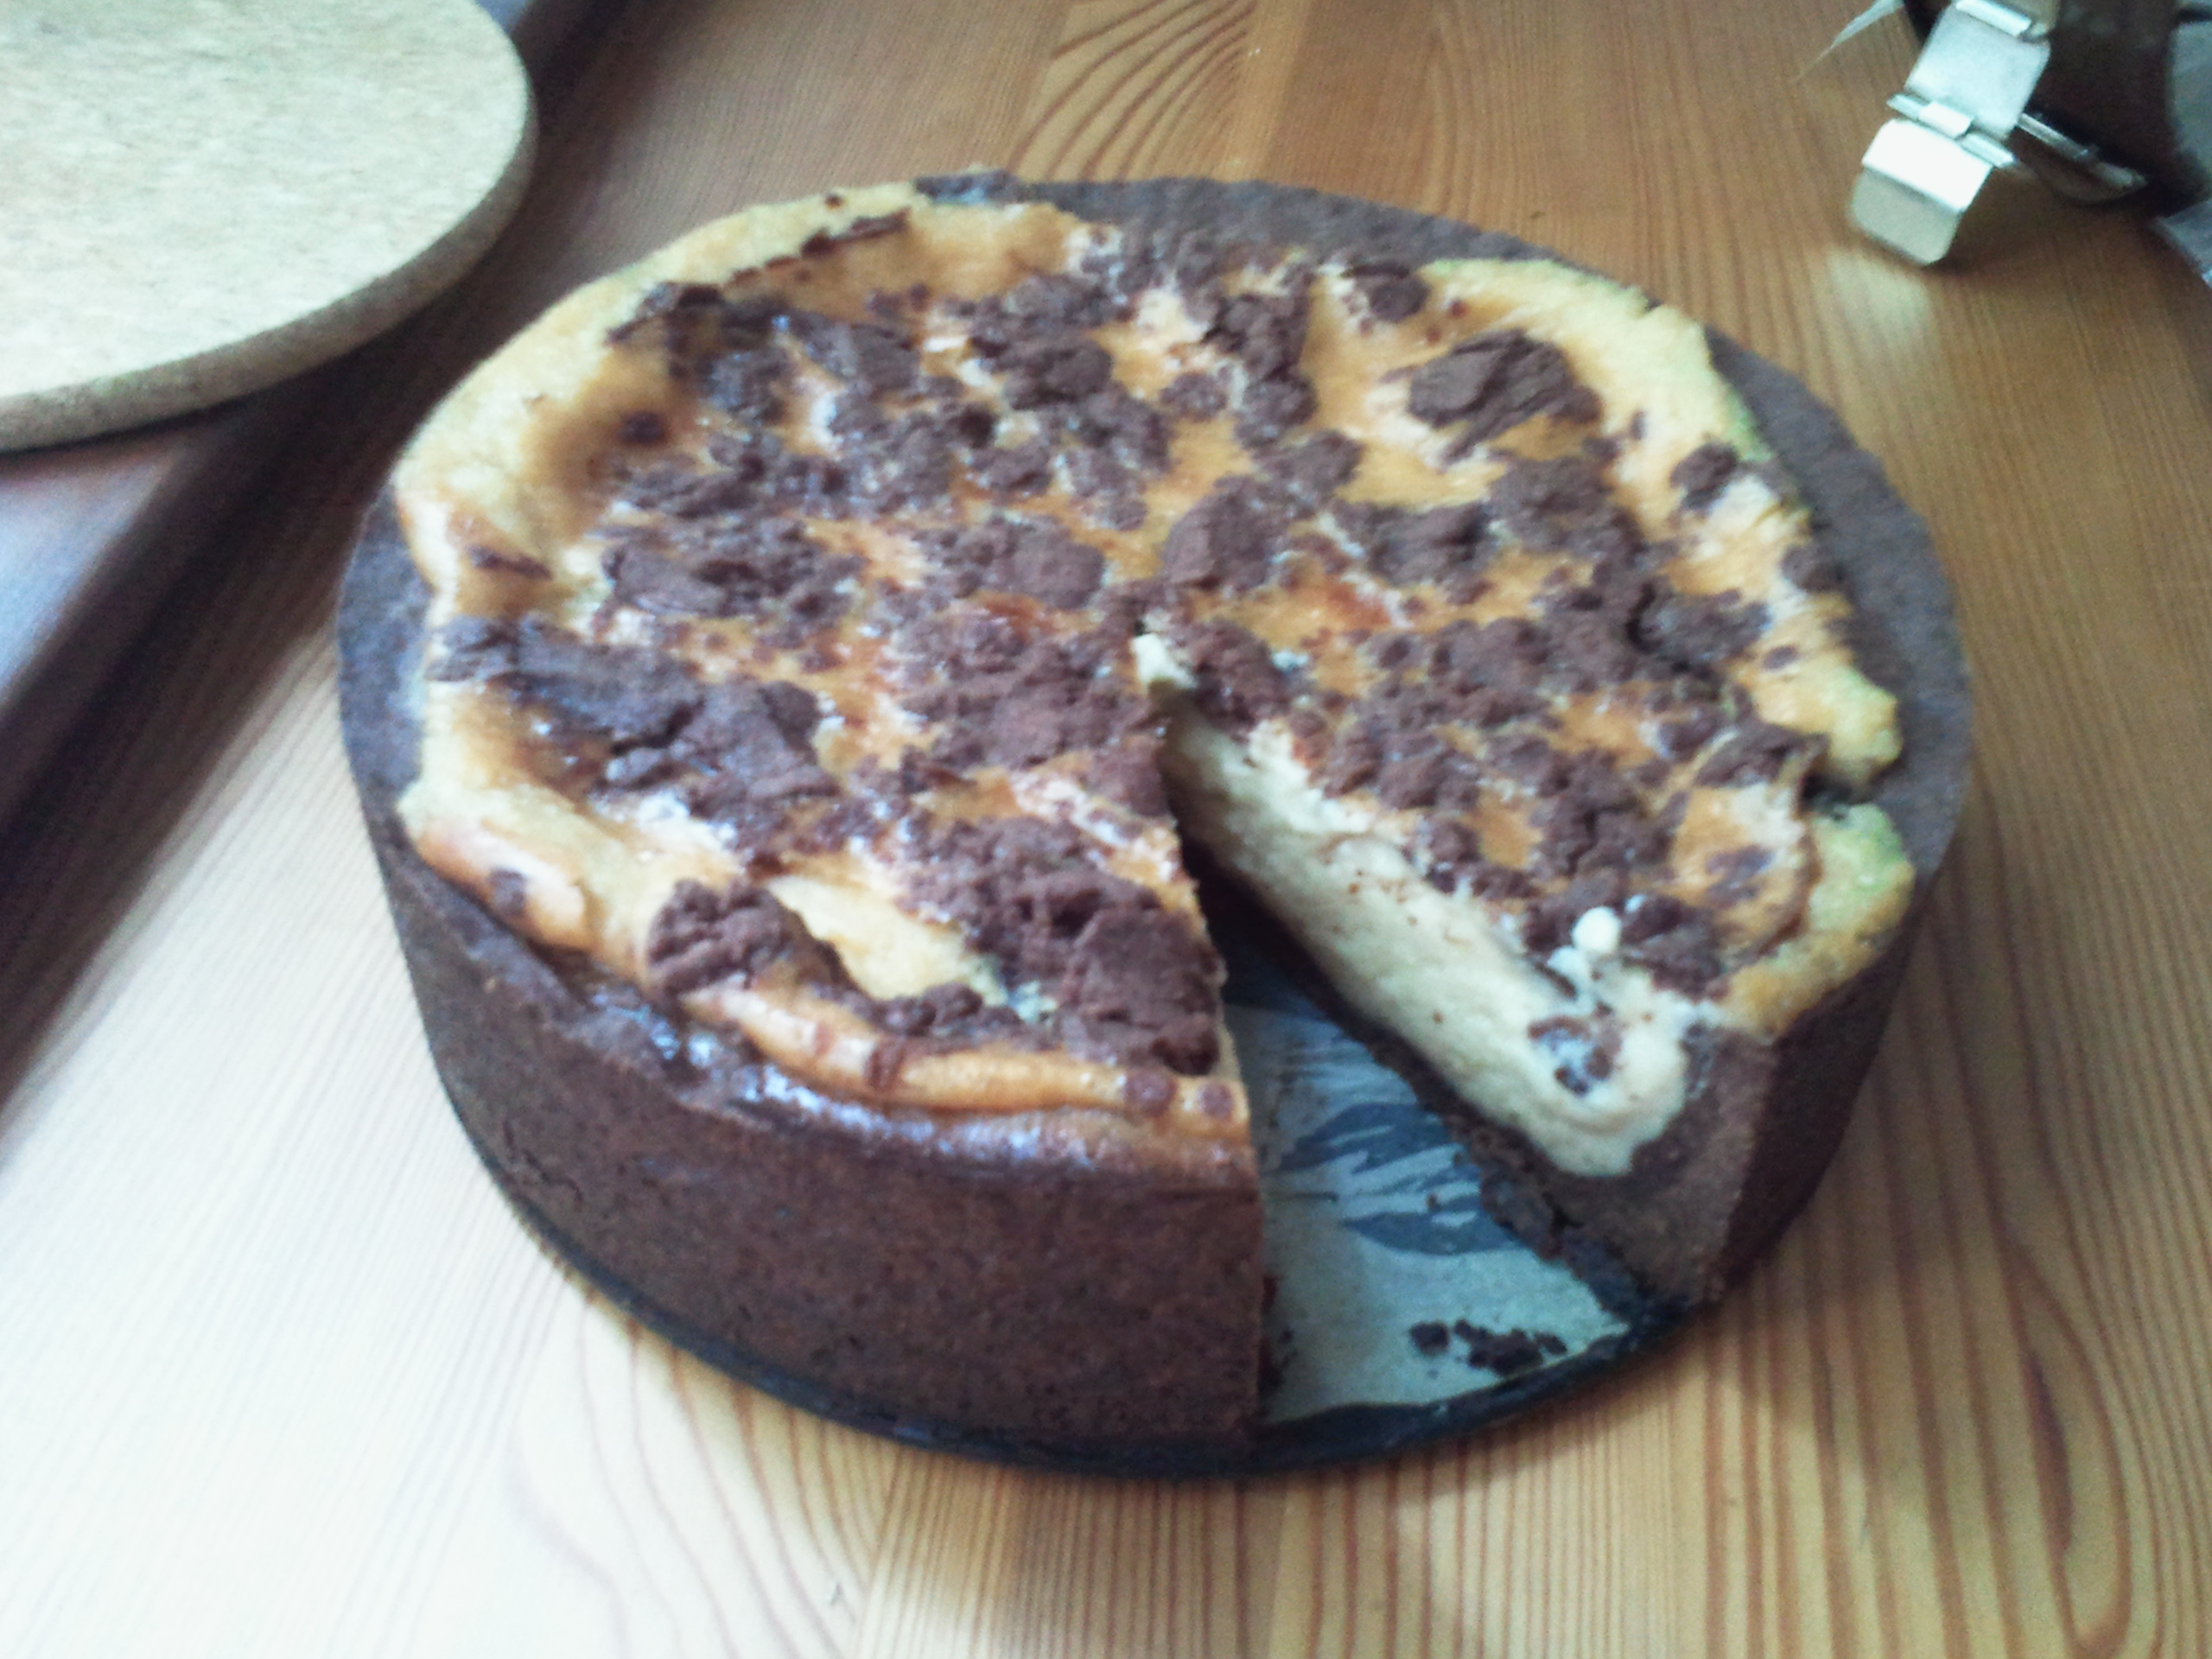
\includegraphics[width=17cm]{img/2012-05-17_10-31-00.jpg}
\end{center}
	\item Nachdem wir die Nutzung von Scala mit Lift beschlo\ss{}en, vereinbarten wir, uns \"uber das Wochenende in den
Framework einzuarbeiten und nachzuvollziehen, wie die Registrierung und Speicherung der angelegten User von statten geht um so
das Grundger\"ust unserer Webseite z\"ugig erarbeiten zu k\"onnen.
	\item Damit dies bei jedem auf gleichem Stand beginnen kann, haben wir einander geholfen die daf\"ur ben\"otigten
Programme und Abh\"angigkeiten einzurichten.
\end{enumerate}
%  \chapter{6.\hspace{0.5em}Woche}\label{wo6}

\section{Prototype}\label{wo6_1}

\begin{enumerate}[label={\Roman*)}]
	\item Zur Einarbeitung in Lift habe ich mehrere Tutorien durchgearbeitet, um so einen kleinen Eindruck \"uber die
M\"oglichkeiten zu erhalten. So habe ich zum Beispiel einen Chat nach Anleitung implementiert, dies ging erstaunlich schnell,
jedoch zeigte dieses Beispiel schon eine gro\ss{}e Schwachstelle dieses Frameworks bez\"uglich unseres Projektes, da sehr wenig
Code ben\"otigt wurde um mehr oder weniger komplexe Funktionen zu implementieren. An sich ist dies eine sehr angenehme und
praktische Tatsache, jedoch kenne ich aus Erfahrung, dass solch ein Framework sehr viel Zeit f\"ur die Einarbeitung ben\"otigt,
leider steht uns im Rahmen des Projektes nicht genug Zeit daf\"ur zur Verf\"ugung.
	\item Am Wochenanfang haben wir dann nocheinmal im Team besprochen wie wir weiter verfahren, da jeder die Erfahrung
gemacht hat, das Lift zwar sehr wenig Code ben\"otigt um komplexe Funktionen zu bieten, aber keiner von uns wirklich verstanden
hatte wie dies in der Tat realisiert wird vom Framework. Aufgrund dieser Tatsache entschieden wir uns den Framework zu wechseln
und haben uns dann in Play 2.0 eingearbeitet.
	\item Auch hierf\"ur richteten wir dann die ben\"otigten Abh\"angigkeiten ein und begannen mit der Implementierung einer
grundlegenden Webseite. Leider kostete uns diese Einsicht sehr viel Zeit, sodass wir nicht die von uns geplanten Aufgaben
umsetzen konnten und im Plan deutlich hinterher h\"angen.
	\item Meine eigentliche Aufgabe dieser Iteration war das Versenden von E-Mails zur Verf\"ugung zu stellen, damit wir
zumindest einen Teil der Benachrichtigungen m\"oglichst fr\"uh nutzen k\"onnen.
	\begin{enumerate}[label={\arabic*}]
		\item Zum Versenden von E-Mails habe ich mich eingelesen, wie unter Linux E-Mails versendet werden k\"onnen.
		\item Nachdem ich lernte, dass diverse Programme zur Verf\"ugung stehen um dies zu bewerkstelligen, entschied ich
mich f\"ur postfix, da dies am einfachsten einzurichten sein sollte und auch neuer ist als die anderen Programme.
		\item Ich bewerkstelligte, von meinem Rechner lokal E-Mails versenden zu k\"onnen, diese landeten aufgrund
fehlender Authentifizierung und Verschl\"u\ss{}elung jedoch im Spam-Ordner der getesteten E-Mailanbieter(Gmail und GMX).
		\item Wenn unsere Website E-Mails versendet, sollten diese jedoch nicht im Spam-Ordner des jeweiligen
Empf\"angers landen, deswegen versuchte ich mittels tls die Authentifizierung zu erm\"oglichen und alle ben\"otigten Zertifikate
bereit zu stellen.
		\item Leider war dies nicht so einfach wie gedacht und gelesen, was auch daran lag, das viele Einstellungen in
der Configdatei, je nach gelesener Quelle, anders eingestellt werden sollten. Es war also leider nicht eindeutig ermittelbar
welche Einstellungen daf\"ur genau ben\"otigt sind.
		\item Diese Probleme endeten mit dem Ergebnis, dass ich in dieser Woche zwar viel Neues dazu gelernt habe, jedoch
kein vorzeigbares Ergebnis bieten konnte. Allerdings habe ich mich auch schon damit besch\"aftigt, welche Plugins oder andere
M\"oglichkeiten es gibt, um mit Scala E-Mails zu versenden, es fehlten also \glqq nur noch\glqq die Grundlagen um es lokal testen
zu k\"onnen.
	\end{enumerate}
\end{enumerate}
%  \chapter{7.\hspace{0.5em}Woche}\label{wo7}

\section{Prototype}\label{wo7_1}

\begin{enumerate}[label={\Roman*)}]
	\item Am Freitag pr\"asentierten Andi und ich unseren bisherigen Stand der Dinge, dies beinhaltete die Registrierung mit
vorhandener Nutzerverwaltung und ein bis dato ausgereiftes Datenbankmodell.
	\item Weil meine zugewiesene Aufgabe nicht, wie geplant, fertig wurde, beriet ich mich mit meinem Team und suchte nach
m\"oglichen L\"osungen. Die von uns pr\"aferierte Variante war, das ich auf dem von Andi bereitgestellten Server entwickel und
somit die Infrastruktur des Servers nutzen kann, auf dem das Versenden von E-Mails problemlos erfolgen kann nach geringf\"ugiger
Konfiguration der Configdatei, auch ohne Authentifizierung, welche lokal ben\"otigt wird.
	\item Nachdem ich mir von Andi die ben\"otigten Zugangsdaten f\"ur eine ssh-Verbindung besorgt habe, fing ich an dort die
Funktionalit\"at der E-Mailversendung zu testen und nach erfolgreichem Test, mit der eigentlichen Implementierung der
E-Mailfunktionalit\"at f\"ur unsere bestehende Anwendung zu beginnen.
	\item Zum Ende der Woche stand dann eine grundlegende Funktion zum Versenden von E-Mails, diese war zwar nicht sehr
ausgereift aber sie lieferte alle geforderten Funktionen. Dies zu bewerkstelligen bedurfte bei mir die gesamte Zeit die ich diese
Woche f\"ur das Projekt eingeplant hatte.
	\item Zum Abschlu\ss{} dieser Woche haben wir uns in der Universit\"at nach Teams separiert getroffen um den jeweiligen
Fortschritt zu besprechen und um weitere Verbesserungsvorschl\"age zu erhalten und das weitere Vorgehen zu besprechen.
	\item Weiterhin haben wir von den Dozenten das Burn-Down-Chart erkl\"art bekommen, um so unseren aktuellen Stand der
Dinge festhalten zu k\"onnen und jederzeit bereit zu sein unseren Stand nach au\ss{}en hin korrespondieren zu k\"onnen.
\end{enumerate}
%  \chapter{8.\hspace{0.5em}Woche}\label{wo8}

\section{Prototype}\label{wo8_1}

\begin{enumerate}[label={\Roman*)}]
	\item Da der letzte von mir gebackene Kuchen sehr gut ankam, entschied ich mich dazu diese Woche wieder einen f\"ur das
Team zu machen, auch um es f\"ur die sehr guten Leistungen des Teams, die sehr zeitaufwendig bearbeitet und abgeschlossen wurden,
trotz immer wieder auftretender Probleme, die, die eigentlich simplen, Aufgaben sehr komplizieren.
	\item Dieses mal entschied ich mich dazu eine Cremetorte zu machen, eigentlich soll es ein K\"asekuchen sein, jedoch
wurde es diesmal eher cremig, wie folgend zu sehen.
\begin{center}
	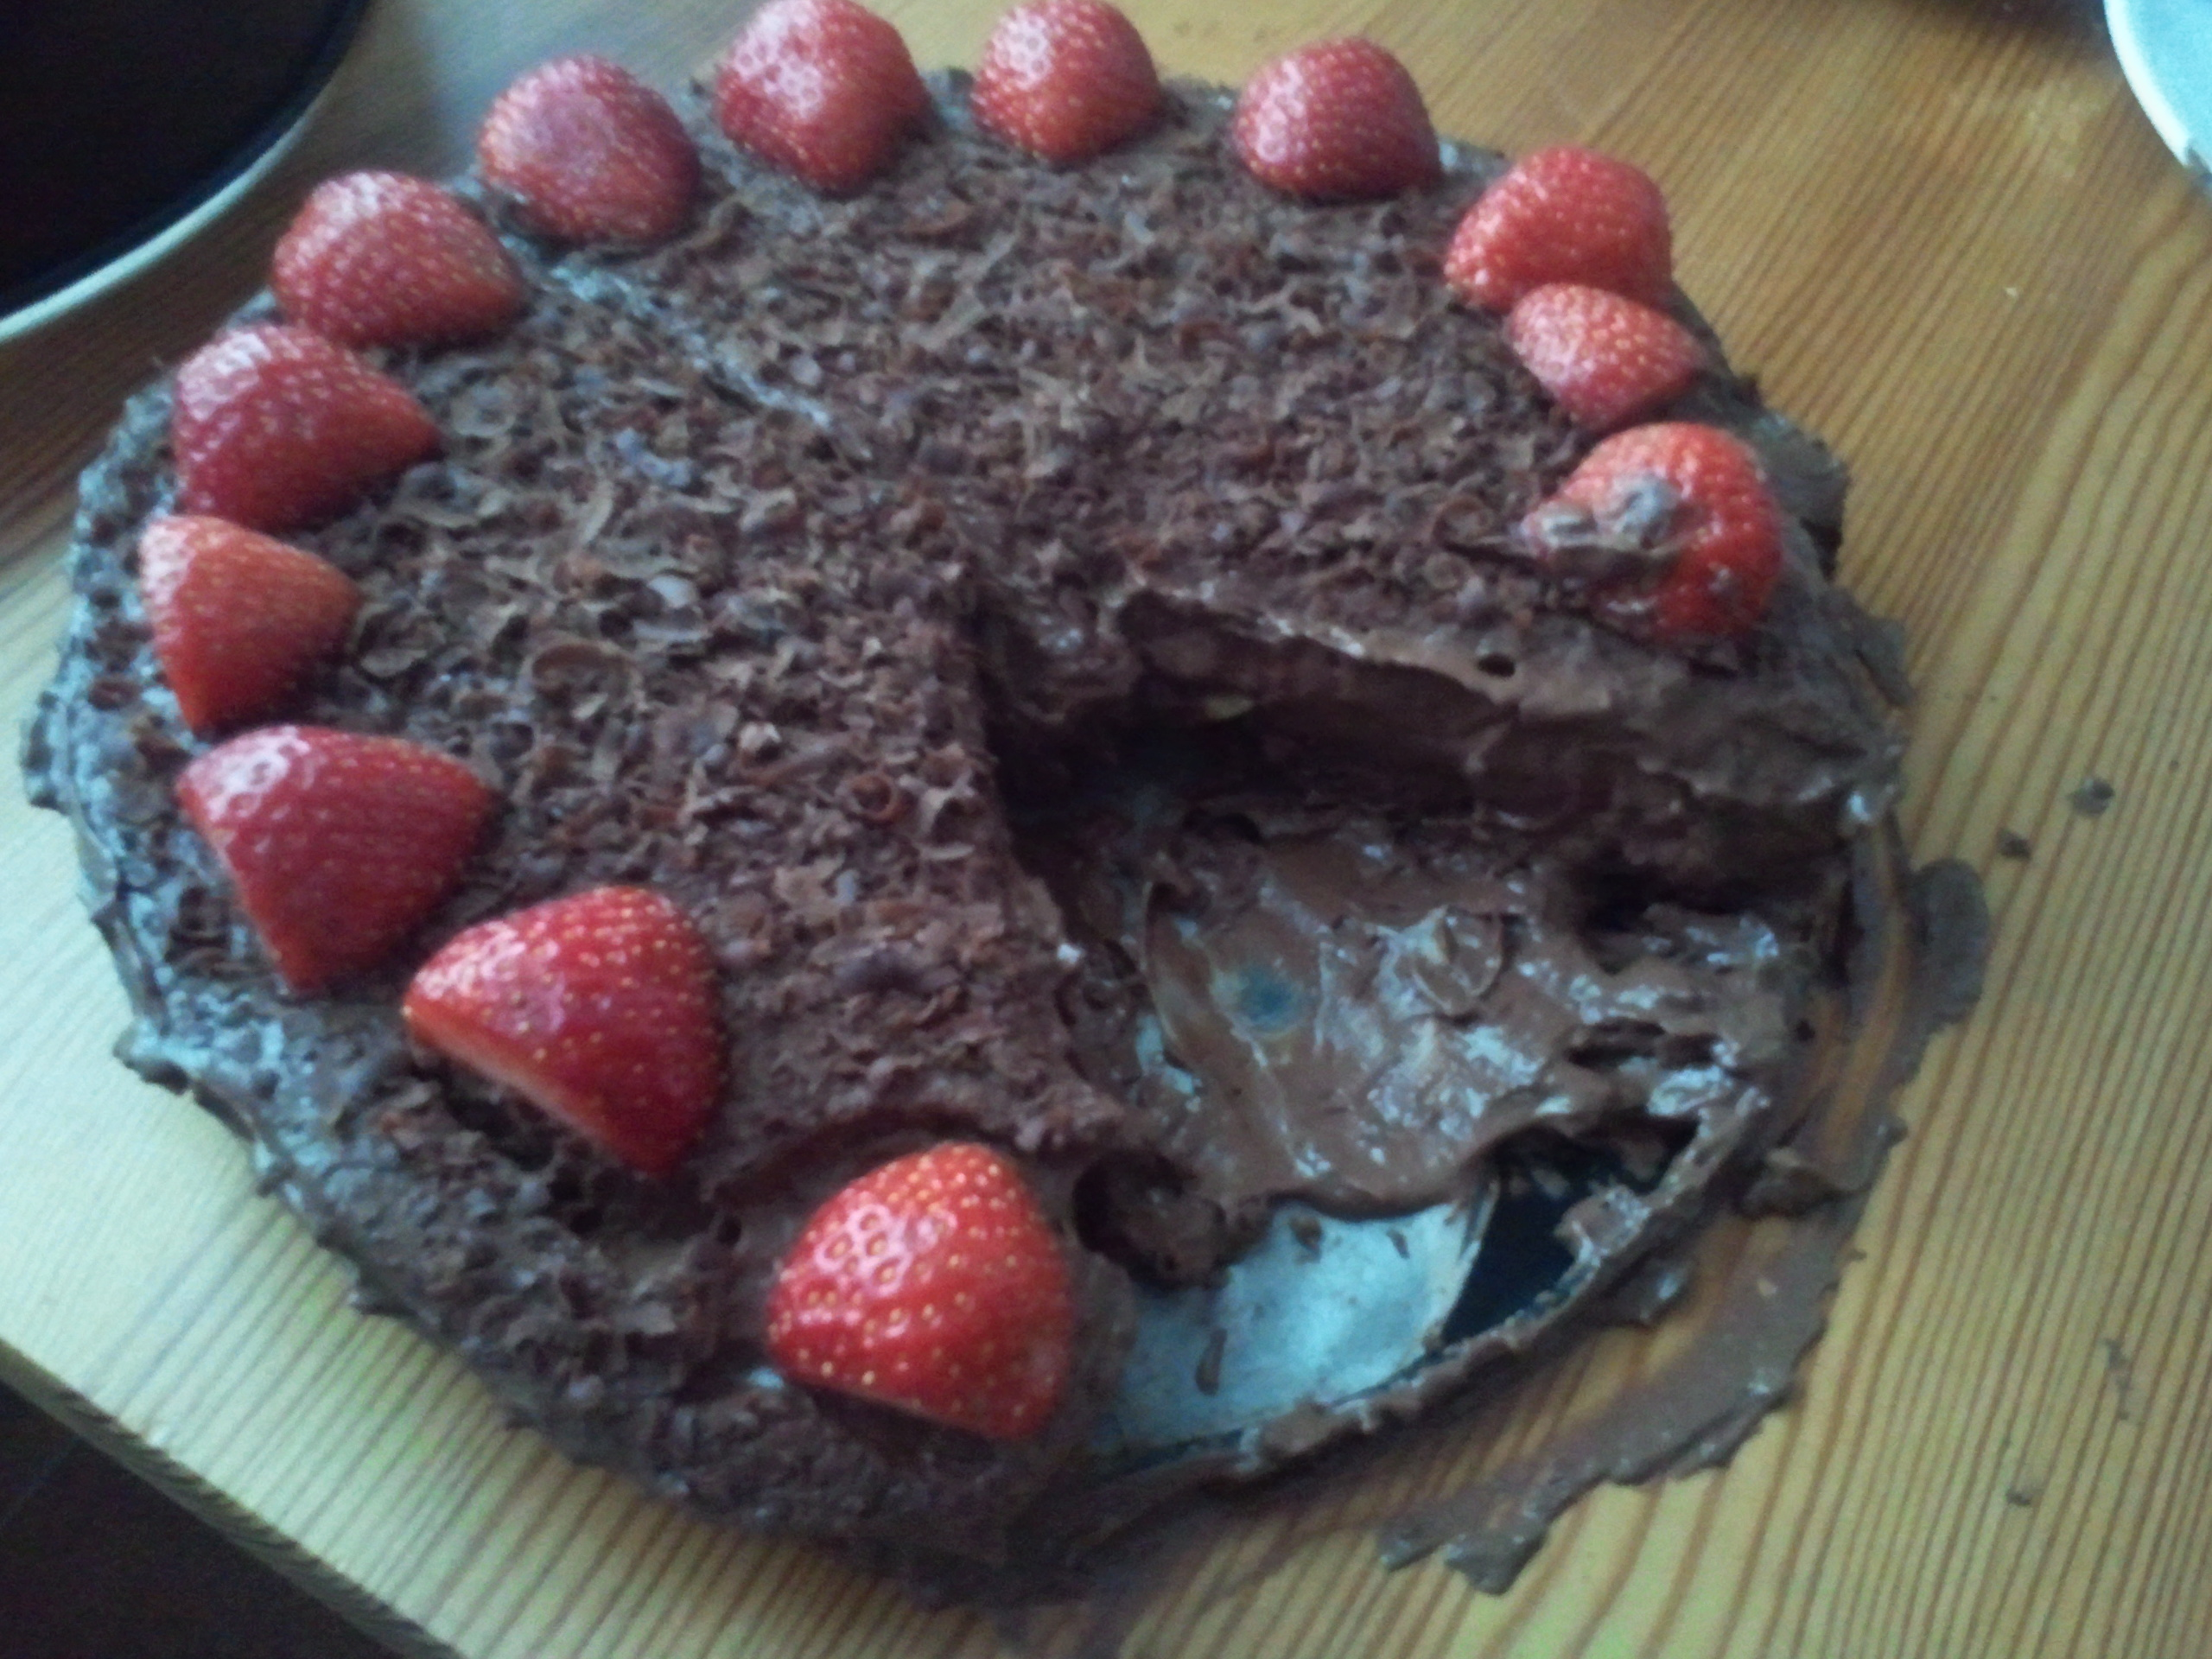
\includegraphics[width=17cm]{img/2012-06-07_10-44-10}
\end{center}
	\item In dieser Woche habe ich die bereits bestehende und funktionierende Funktion der E-Mailversendung weiter ausgebaut
und den gestiegenen Anwendungsf\"allen angepasst.
	\item Weiterhin habe ich mich mit dem Team um die Zuteilung der neuen Aufgaben gek\"ummert, sodass jeder seine zu
bearbeitenden Aufgaben hat und wei\ss{} was zu tun ist.
	\item Mir wurden als neue Aufgaben die Ermittlung der favorisiten aus den bestehenden Touren und das Ermitteln der
initialen Templates f\"ur Touren zugewiesen.
	\item Damit ich meine Aufgaben m\"oglichst zeitnah erledigen kann und es nicht wieder auf den letzten Dr\"ucker
geschieht, wie in der Vergangenheit leider manchmal passiert, habe ich angefangen mich mit dem Thema des Caching intensiv zu
besch\"aftigen und schon im Zusammenhang mit Scala geguckt was dort m\"oglich ist.
	\item Am Freitag haben wir uns in der Universit\"at getroffen und es wurde spontan entschieden, dass Treffen nach
drau\ss{}en auf die Wiese zu verlegen. Dies erheiterte die Stimmung des Treffens, was dem gesamten Verlauf sehr gut entsprach, da
dieses Treffen sehr locker aufgebaut war und es nur um den aktuellen Stand der Gruppen ging, somit war dieses Treffen
allgemein entspannend aufgebaut und verlief sehr angenehm, dies empfand ich als besonders wohltuend f\"ur den allgemeinen Ablauf
des Projektes, da es so nicht zu sehr zu einer enormen Programmieraufgabe wird bei der am Ende ein fertiges Projekt erwartet wird
und nicht auf die Bed\"urfnisse der Studierenden eingegangen wird.
	\item Diese Woche habe ich mich mit dem Team 4 in Verbindung gesetzt, um eine m\"ogliche Zusammenarbeit bereits vor Ende
des Projektes zu erm\"oglichen. Dabei ist geplant, dass von Seiten des Teams 4 aus bei uns automatisch Touren generiert werden,
wenn dort bei einer Planung einer Reise eine Taxifahrt enthalten ist.
\end{enumerate}
%  \chapter{9.\hspace{0.5em}Woche}\label{wo9}

\section{Prototype}\label{wo9_1}

\begin{enumerate}[label={\Roman*)}]
	\item Ich habe die Ermittlung der Favoriten aus den bestehenden Touren implementiert und mich damit besch\"aftigt welche
M\"oglichkeiten es zum Caching gibt. Letztendlich habe ich mich f\"ur die von Play 2.0 mit EHCache bereitgestellte
Standardversion entschieden und dieses implementiert. Dabei ist allerdings noch ausstehend, inwiefern der Cache funktioniert, da
dies nur im Feldtest wirklich ersichtlich wird.
	\item Ich habe mir Gedanken zur Neuverteilung der Aufgaben, welche Tu zugewiesen waren, gemacht, da dieser das Projekt
kurzfristig und unerwartet verlassen hat. Dies wirft unser gesamtes Team leider sehr zur\"uck, da die Aufgabe der automatischen
Bestellung und das Kl\"aren mit MyTaxi ob dies in Wolfsburg verf\"ugbar sein wird zugewiesen war.
	\item Weiterhin habe ich die initialen Templates f\"ur Touren aus der Vorgabe der FE-Taxiliste in die Datenbank
\"ubernommen und diese werden nun zusammen mit den Favoriten ermittelt, dabei werdern zuerst die Favoriten bestimmt und wenn
diese nicht ausreichend sind, werden weitere Templates aus der FE-Taxiliste zugef\"ugt bis die gew\"unschte Anzahl(8 Templates)
erreicht ist und somit eine gen\"ugend gro\ss{}e Auswahl an sofort w\"ahlbaren Templates bereit steht. Sollten jedoch noch keine
Favoriten bestehen, so werden nur die Templates aus der FE-Taxiliste angezeigt.
\end{enumerate}
\end{document}